\chapter{Data}
\label{chap:data}
% \thispagestyle{fancy}
This chapter discusses the datasets used in the thesis, as well as the processing steps to make the data more learnable. The main dataset used in the thesis is \textit{Human3.6M}: Large Scale Datasets and Predictive Methods for 3D Human Sensing in Natural Environments \cite{H3.6}. Most of the related works benchmark their methods on Human3.6M and it also is freely accessible to academics on request. For further evaluation of model performance in the wild, outdoor datasets that do not have 3D ground truth such as \textit{3DPW}: 3D Poses in the Wild \cite{3dpw} would be used.

\begin{figure}[h]
    \centering
    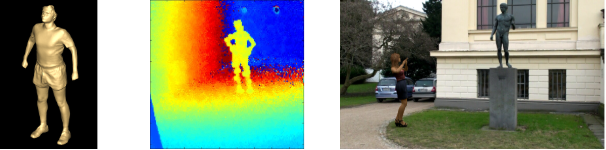
\includegraphics[width=\textwidth]{figures/h36/modlities.png}
    \caption{Full body model, depth from time of flight and mixed reality in Human3.6M dataset}
    \label{fig:h36_modality}
\end{figure}

\section{Human3.6M}
Human3.6M is a large scale indoor dataset with 3.6 million human poses collected with 4 cameras at different angles using a highly accurate maker-based \ac{mocap} system. The dataset constitutes 15 diverse motion and actions such as eating, sitting, walking in various everyday scenarios such as a hand in the pocket, talking over the phone, walking a dog, etc. These actions are performed by 11 professional actors wearing a variety of realistic clothing. The datasets provides synchronised 2D and 3D data including full-body scans as shown in figure[\ref{fig:h36_modality}]. It also includes mixed-reality test data created using animated human models to cover huge variations of background, clothing, illumination, occlusion, and camera angles.

% TODO -- Add things related to 3D projection, depth ambiguity, rigid body alignment
% \section{3D Geometry}
% \lipsum[1-4] %FIXME

% \subsection{Camera projection}
\section{Depth Ambiguity and Camera Modeling}

The projection of the poses in the thesis is using a simple pinhole camera model as illustrated in fig.\ref{fig:pinhole}. A unit camera model is assumed for the dataset and the poses are predicted around the origin and translated to a fixed image plane. Thus the error in projection is not significant. 

\begin{figure}[!h]
    \centering
    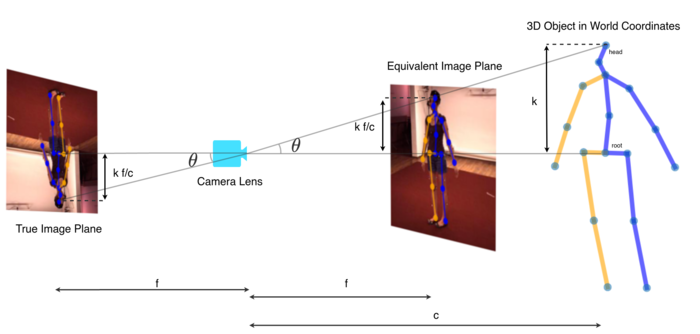
\includegraphics[scale=0.4]{figures/background/pinhole.png}
    \caption{Pinhole Camera Model. Image Source \cite{pinhole}}
    \label{fig:pinhole}
\end{figure}

One of the main problems discussed in \ref{section:Related Work} is depth ambiguity. The fig \ref{fig:depthambi} illustrates the challenges in lifting 2D pose to 3D pose. During evaluation under protocol 2, the 3D poses are transformed using rigid or Procrustes alignment with the ground truth pose as illustrated in fig. \ref{fig:procrustes}. But in the proposed method we only translated and rotate but do not scale the pose.



%FIXME protocol 2 or both protocols + scaling explanation


\begin{figure}[!h]
    \centering
    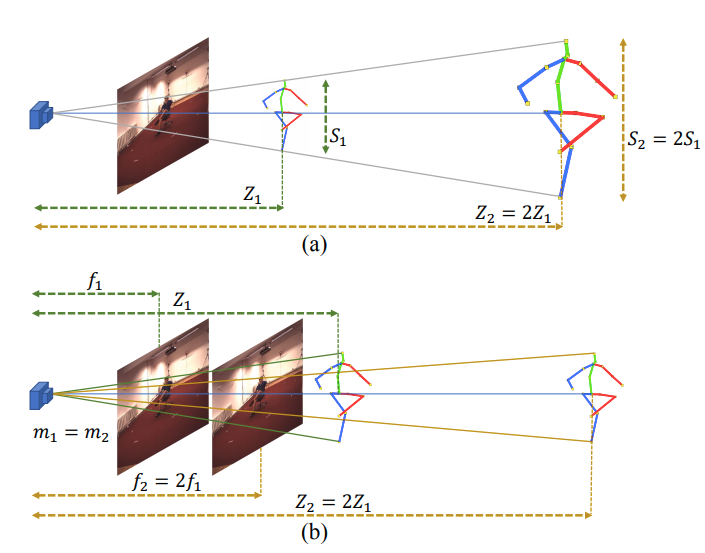
\includegraphics[scale=0.4]{figures/background/depthambi.png}
    \caption{Illustration of depth ambiguity. (a) shows 2 of the infinite possible poses that result in the same 2D reprojection. Where (b) shows the same phenomenon for different focal legths
    Image Source \cite{poselifter}}
    \label{fig:depthambi}
\end{figure}



%FIXME explain properly
%FIXME fix citation of pinhole



% % \lipsum[1] %FIXME
% \subsection{Depth Ambiguity and Camera Modeling}


% % \lipsum[1] %FIXME
% \subsection{Procrustes Alignment}
% % \lipsum[1-4] %FIXME


\section{Processing}

The methods explored by this thesis would require only images, 2D, and 3D human pose from the dataset. The following are the pre-processing steps for the 2D and 3D poses.


% \begin{figure}[!h]
%     \centering
%     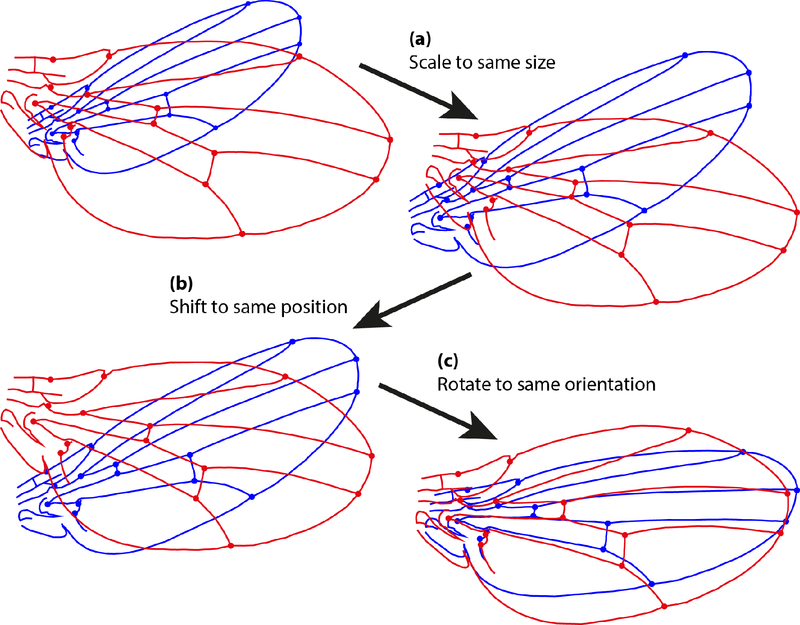
\includegraphics[scale=0.8]{figures/background/Procrustes_superimposition.png}
%     \caption{Illustration of Procrustes Alignment. Image Source \cite{Procrustes}}
%     \label{fig:procrustes}
% \end{figure}

\begin{figure}
    \centering
    \begin{subfigure}[b]{0.25\textwidth}
        \centering
        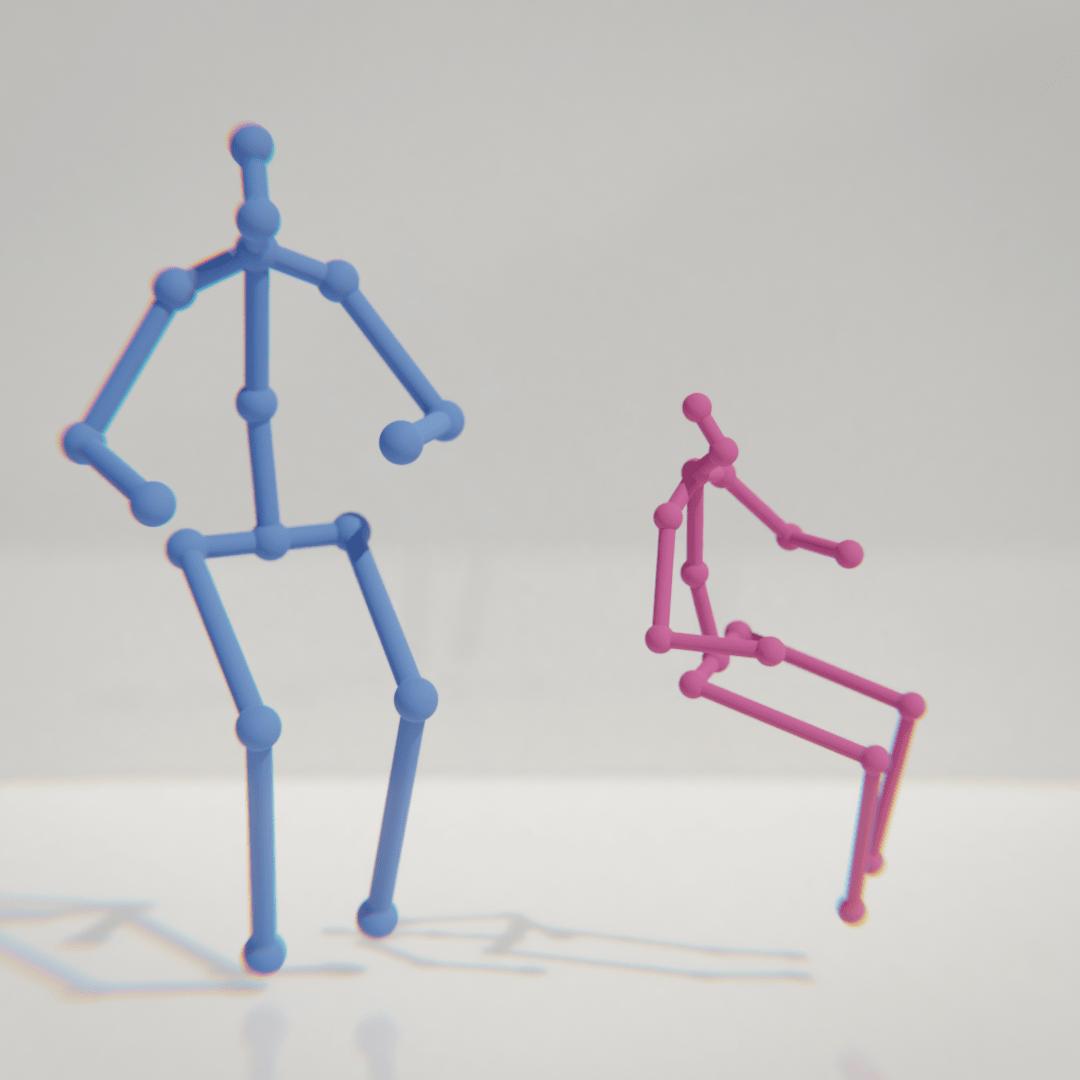
\includegraphics[width=\textwidth]{figures/h36_viz/proc_raw.png}
        \caption{$y=x$}
        \label{fig:y equals x}
    \end{subfigure}
    \hfill
    \begin{subfigure}[b]{0.25\textwidth}
        \centering
        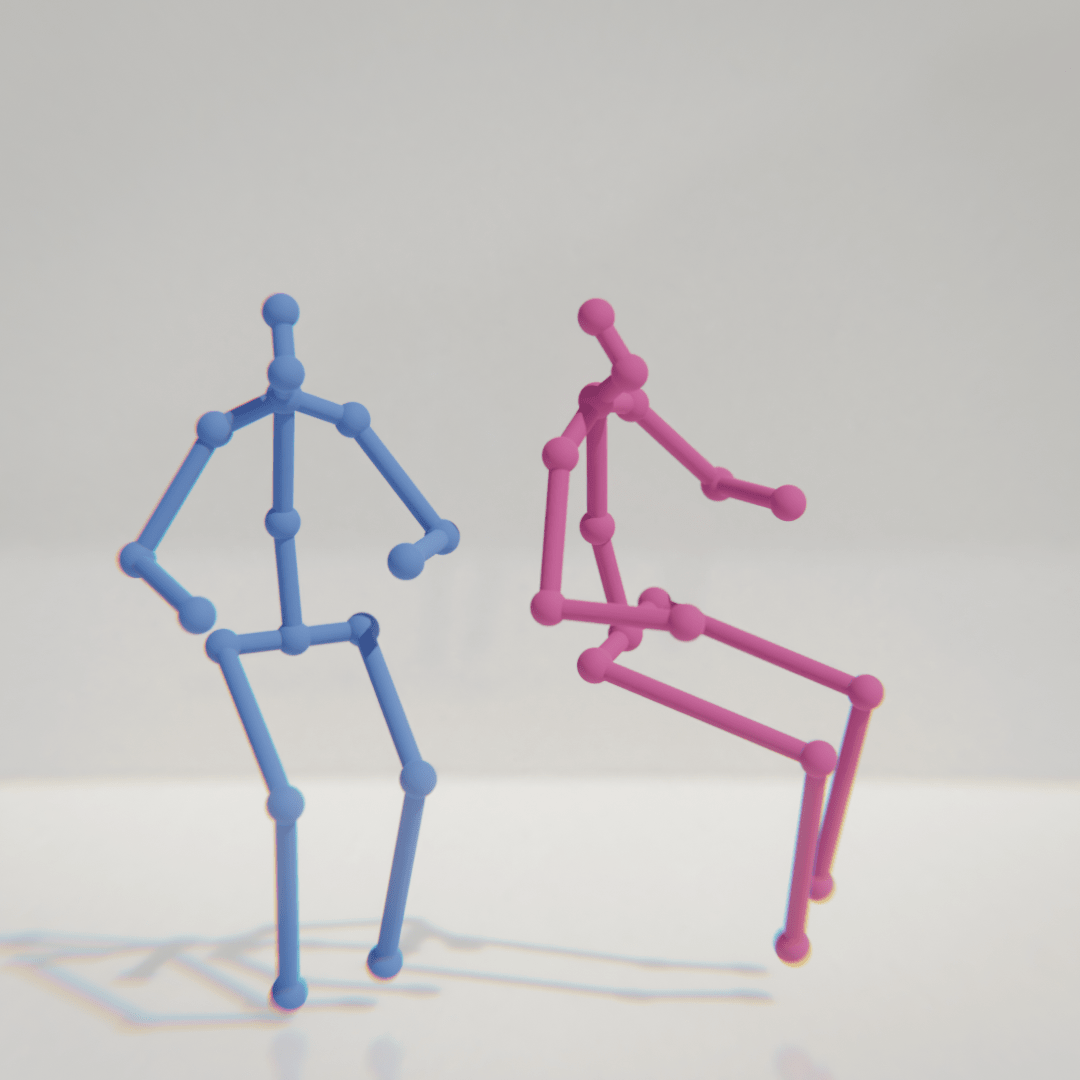
\includegraphics[width=\textwidth]{figures/h36_viz/proc_scale.png}
        \caption{$y=3sinx$}
        \label{fig:three sin x}
    \end{subfigure}
    \hfill
    \begin{subfigure}[b]{0.25\textwidth}
        \centering
        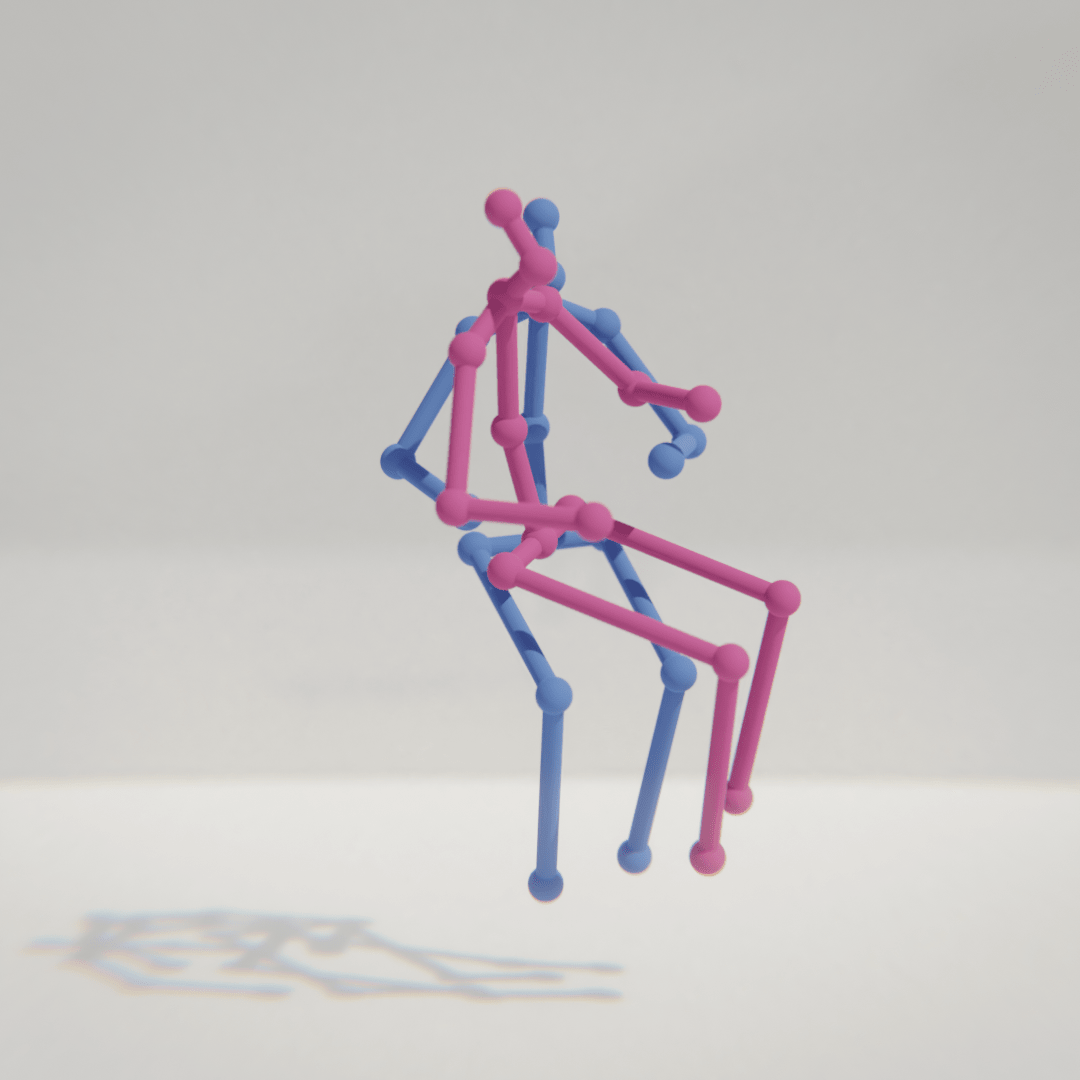
\includegraphics[width=\textwidth]{figures/h36_viz/proc_pos.png}
        \caption{$y=5/x$}
        \label{fig:five over x}
    \end{subfigure}
    \hfill
    \begin{subfigure}[b]{0.25\textwidth}
        \centering
        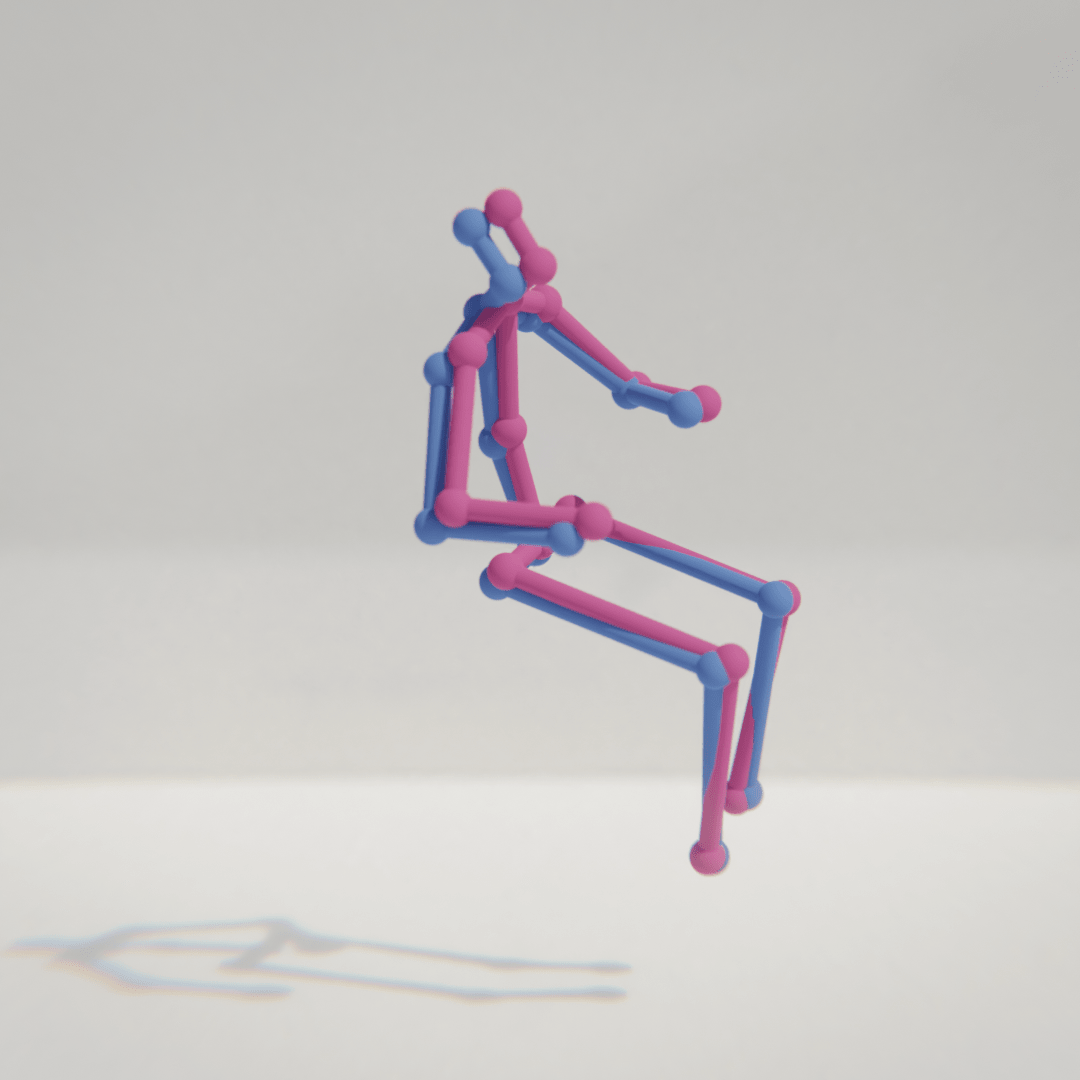
\includegraphics[width=\textwidth]{figures/h36_viz/proc_rot.png}
        \caption{$y=5/x$}
        \label{fig:five over x}
    \end{subfigure}
    \caption{Three simple graphs}
    \label{fig:procrustes}
\end{figure}

The 3D pose in the dataset that is obtained from the marker-based \ac{mocap} is in a global reference frame. These poses using the camera parameters are transformed into the camera coordinate frame. For the task of predicting 3D pose from either images or 2D pose, it is unrealistic to directly estimate all the joints of the pose in a global frame. So the first step of processing would be to zero the pose w.r.t the root joint say, Pelvis. As the root is always zero, we remove it so we do not have to learn the constant joint. Removing Pelvis, 16 out of the 17 joints or keypoints remain. The 3D pose is further scaled in down so that the distance between the root and the head is 1. This results in numerical stability during training.

\begin{figure}[h]
    \centering
    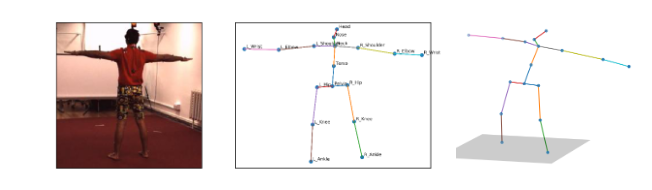
\includegraphics[width=\textwidth]{figures/h36_viz/h36poses.png}
    \caption{Human3.6M Pose Sample}
    \label{fig:h36_poses}
\end{figure}

The 2D pose which is obtained from the 3D pose, is also in the camera coordinate frame. The 2D pose is also zeroed and scaled so that the distance between the root and head is 1/c units. Where c is a constant distance at which the image plane is fixed. As a unit camera or camera with unit focal length is assumed the projection of unit 3D poses onto a plane at a fixed distance of 1/c units. The root of the 2D pose is however removed to remain consistent with the 3D pose. An image sample from the dataset with its corresponding 2D and 3D pose is illustrated in the figure[\ref{fig:h36_poses}].

% TODO update - experiments are yet to be done
% TODO link MPJPE to its explanation in other chapter or sections

The estimated poses from the networks that are trained on downscaled poses are upscaled to the original size using for valuation. This postprocessing step is required for getting the distance between prediction and ground truth keypoints in true units of millimeters.

